\section{Estruturando a Aplicação}
%---------------------------------------------------------------------[ Início ]
\begin{frame}[fragile,t]{Criando Um Helper}
    \begin{itemize}
      \item  Um helper será criado para promover o reúso e evitar a repetição 
        de código em uma aplicação. 
    \end{itemize}
      \begin{lstlisting}[style=RubyInputStyle, basicstyle=\tiny\ttfamily, firstline=1, lastline=10, caption=app/helpers/application\_helper.rb]
module ApplicationHelper
    def preenche_titulo(titulo_da_pagina='')
        titulo_padrao="Blog App"
        if (titulo_da_pagina.empty?)
            titulo_padrao
        else
            "#{titulo_da_pagina} | #{titulo_padrao}"
        end
    end
end
      \end{lstlisting}
\end{frame} 
%---------------------------------------------------------------------[ Início ]
\begin{frame}[fragile,t]{Estruturando a Aplicação}
    \begin{itemize}
      \item  Uma aplicação web deve ser estruturada de forma a facilitar o seu uso.
        Uma ferramentas utilizadas para isso é o protótipo essencial. A ideia inicial
        para a aplicação Blog foi pensada. 
      \begin{figure}[h!]
        \centering
        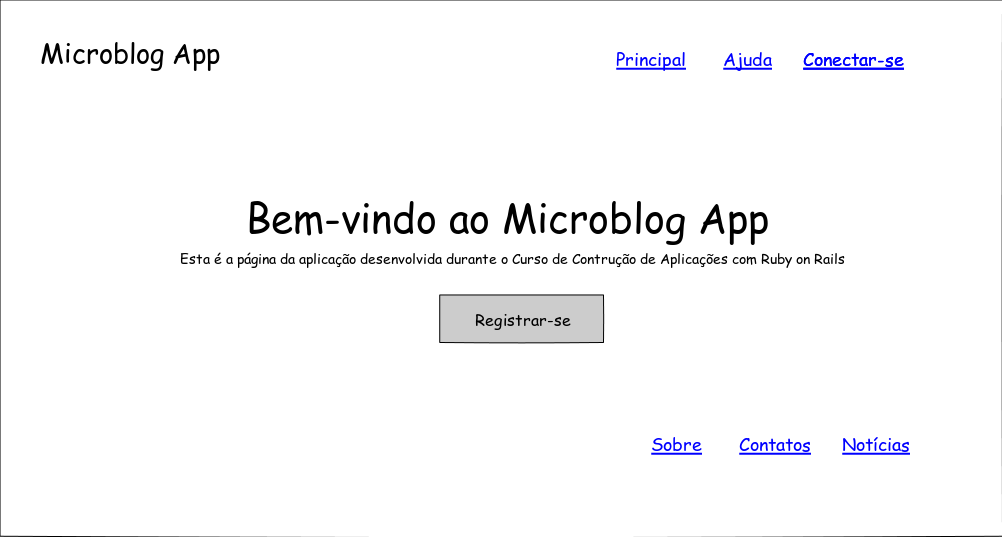
\includegraphics[width=0.65\textwidth]{imagens/esboco-da-pagina-principal.png}
      \end{figure}
    \end{itemize}
\end{frame} 

%---------------------------------------------------------------------[ Início ]
\begin{frame}[allowframebreaks, fragile,t]{Navegação da Aplicação}
      \begin{lstlisting}[style=RubyInputStyle, basicstyle=\tiny\ttfamily, caption=app/views/layouts/application.html.erb]
<!DOCTYPE html>
<html>
<head>
  <title><%= preenche_titulo(yield(:titulo)) %></title>
  <%= stylesheet_link_tag    'application', media: 'all', 
      'data-turbolinks-track' => true %>
  <%= javascript_include_tag 'application', 'data-turbolinks-track' => true %>
  <%= csrf_meta_tags %>
</head>
<body>
  <%= link_to "Blog", "#", id: "logo" %>
  <p>
    <ul>
      <li><%= link_to "Index", home_index_path %></li>
      <li><%= link_to "Help", home_help_path %></li>
    </ul>
  </p>
  <%= yield %>
</body>
</html>
      \end{lstlisting}
\end{frame} 

%---------------------------------------------------------------------[ Início ]
\begin{frame}[allowframebreaks, fragile,t]{Refatorando as Páginas Index e Help}
   \begin{lstlisting}[style=RubyInputStyle, basicstyle=\tiny\ttfamily, caption=app/views/home/index.html.erb]
<%= provide :titulo, "Index" %>
<div>
    <h1>Blog App</h1>
    <p>
      Esta e a pagina principal da aplicacao Blog desenvolvida durante 
      o Laboratorio de Engenharia de Software.
    </p>
    <%= link_to "Posts", posts_path %>
</div>      
  \end{lstlisting}
  
   \begin{lstlisting}[style=RubyInputStyle, basicstyle=\tiny\ttfamily, caption=app/views/home/help.html.erb]
<%= provide :titulo, "Help" %>
<div>
    <h1>Blog App</h1>
    <p>
      Esta e a pagina de ajuda da aplicacao Blog desenvolvida durante 
      o Laboratorio de Engenharia de Software.
    </p>
</div>      
  \end{lstlisting}
\end{frame} 

%%-------------------------------------------------------------------------------------- Início
\begin{frame}[allowframebreaks, fragile,t]{Hora de Colocar a Mão na Massa}
	\begin{enumerate}
		\item Implemente os recursos aprensentados na aula de hoje.		
		\item Registre as mudanças realizadas no repositório local:
		\begin{lstlisting}[style=BashInputBasicStyle]
			$ git add .
		\end{lstlisting}

        \item Efetive as mudanças realizadas no repositório local:  		
        \begin{lstlisting}[style=BashInputBasicStyle]
			$ git commit -m "#1: manutencao de posts"
		\end{lstlisting}

		\item Registre as alterações no repositório remoto:
		\begin{lstlisting}[style=BashInputBasicStyle]
			$ git push -u origin master
		\end{lstlisting}
	\end{enumerate}
\end{frame}